\begin{figure}[!htbp]
\centering
\begin{subfigure}{0.49\textwidth}
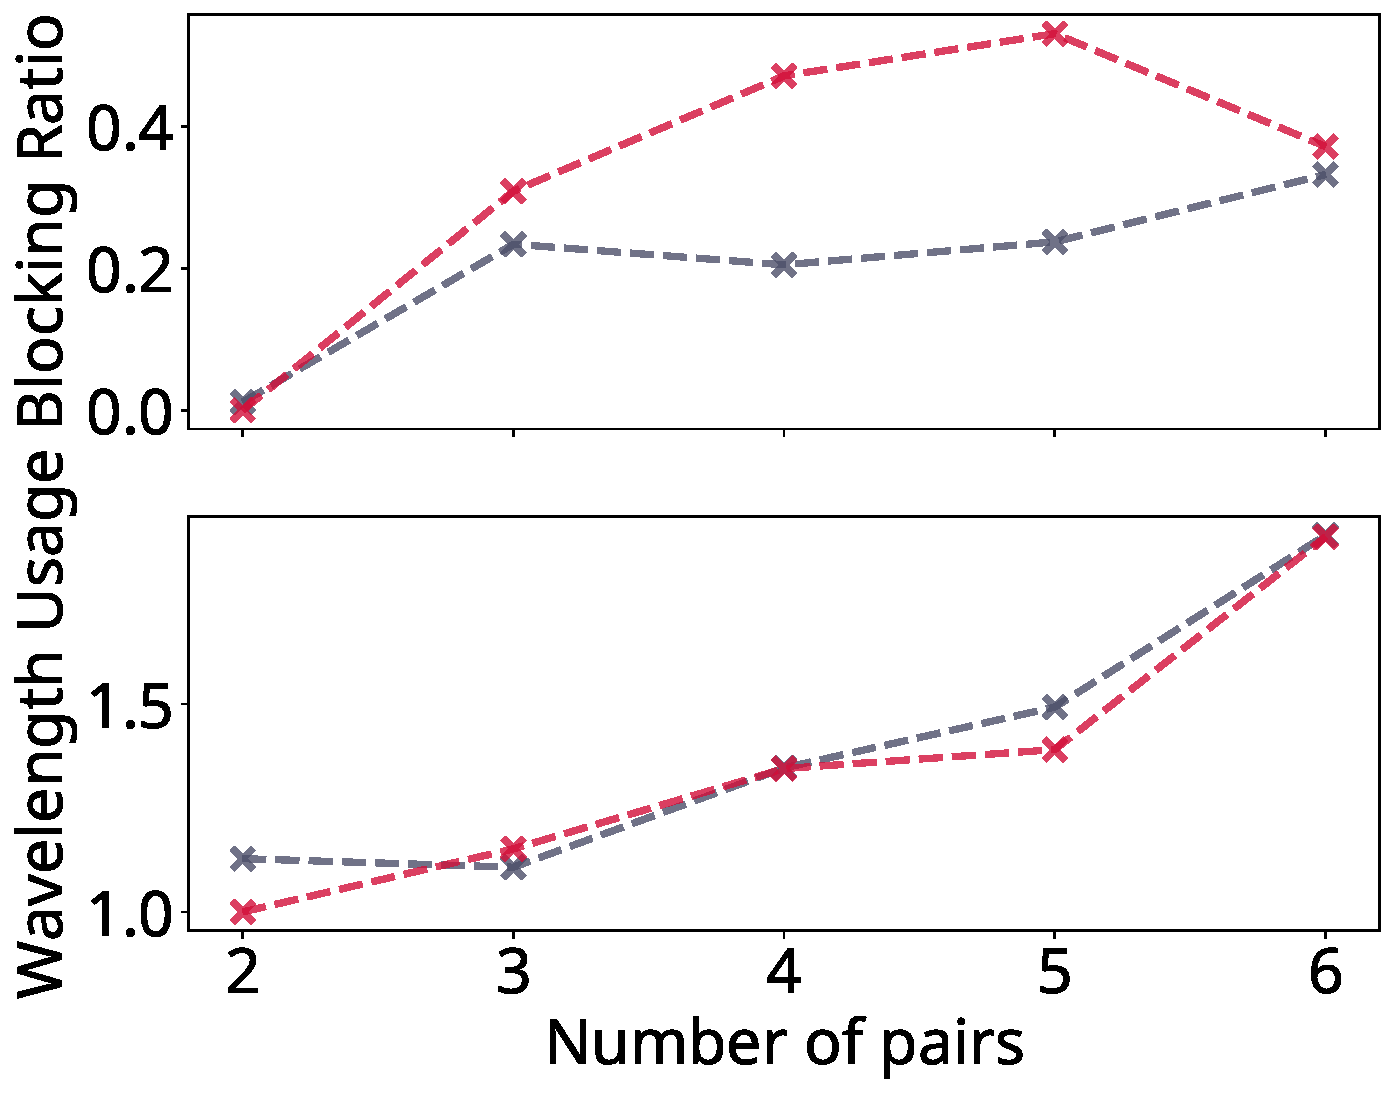
\includegraphics[width=\textwidth]{pictures/plots/rawa/n_pairs/x-2-2-s.pdf}
	\caption{$\abs{P}=2, \abs{\Lambda} = 2$, small topology}
\end{subfigure}
\begin{subfigure}{0.49\textwidth}
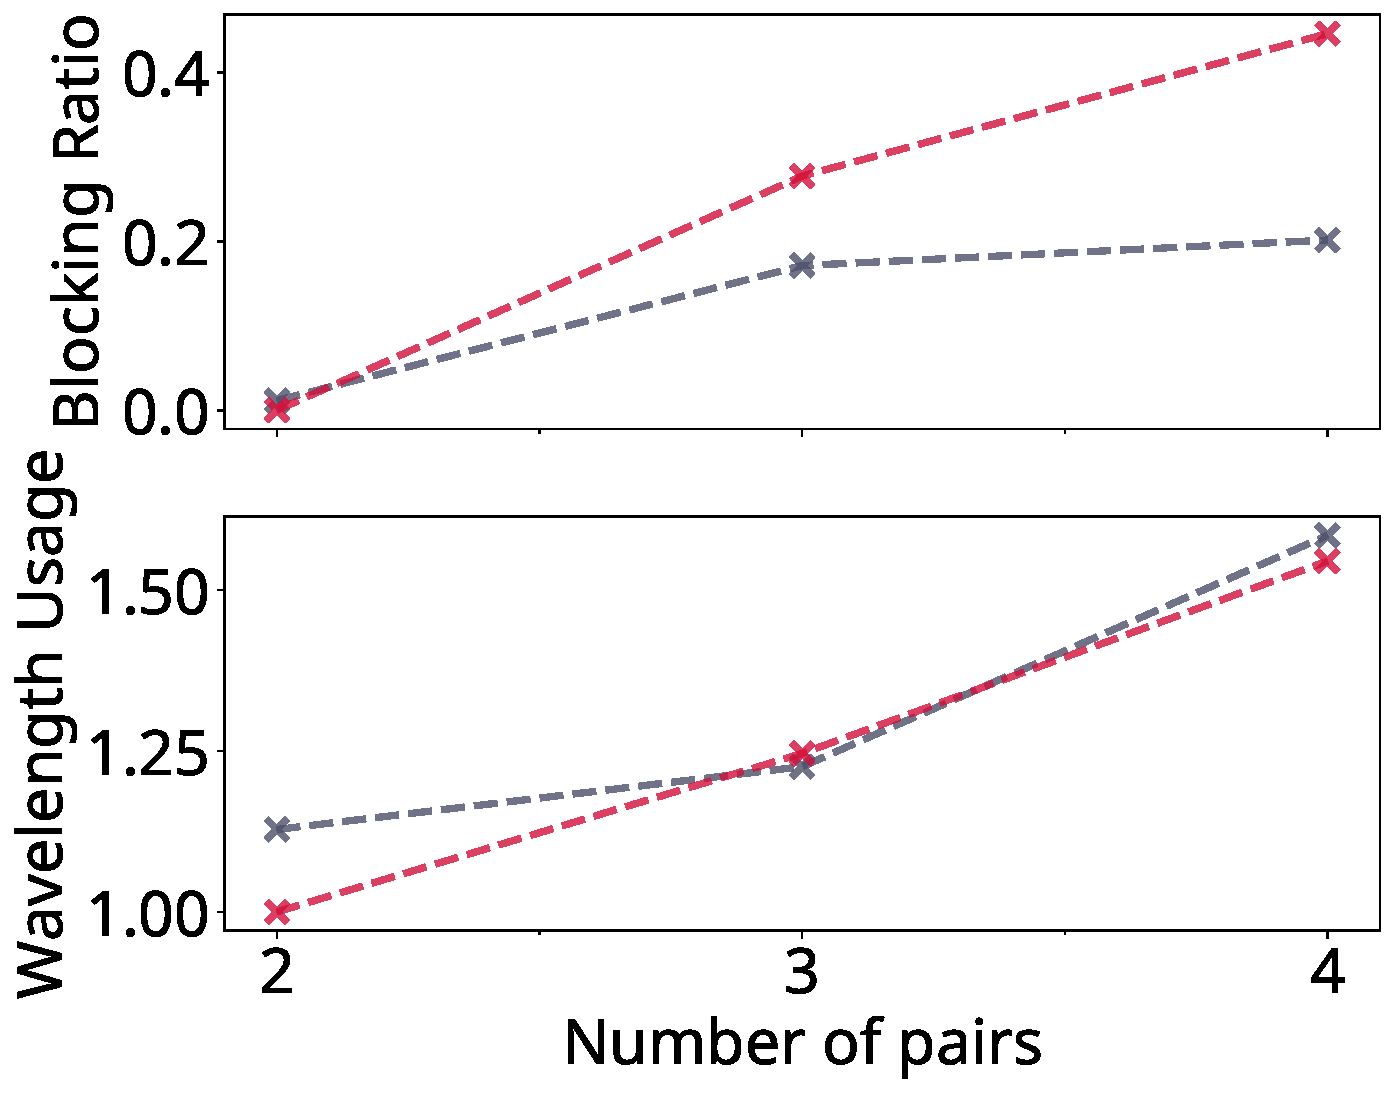
\includegraphics[width=\textwidth]{pictures/plots/rawa/n_pairs/x-2-3-s.pdf}
	\caption{$\abs{P}=2, \abs{\Lambda} = 3$, small topology}
\end{subfigure}
\caption{%The blocking probability and number of wavelength used.
\protect\reddashed is the joint RWA formulation, and 
\protect\blackdashed is the two-steps formulation.
}
\label{fig:rawa}
\end{figure}
